\documentclass[12pt,a4paper]{article}
\usepackage[latin1]{inputenc}
\usepackage{graphicx}
\usepackage{amsfonts}
\title{A software to generate evenly spaced points on the unit N-simplex}
\author{Gianfranco Giulioni}
\begin{document}
\maketitle
\section*{Installation}
This application has been written in Java. It is platform independent and it does not need a special installation procedure. 

To run the application, you must have a properly installed Java Runtime Environment (JRE). In the case your system is endowed with a JRE, the \verb+java+ command is accepted by your command line. 

If not you must install the JRE. To this aim, if your operating system has a software packages manager, you should first check for the existence of the java standard edition package and eventually install it from the software packages manager. If not, the JRE can be freely downloaded from the web. At the present time it is available from 

\verb+ http://www.oracle.com/technetwork/java/javase/downloads/index.html +

Please, read also the installation instruction provided in the download page.

Now, the \verb+java+ command is available to your system.

To install the application,
\begin{itemize}
\item download the \verb+simplex.zip+ file from

\verb+ http://erre.unich.it/giulioni/simplex.zip+


\item create a folder; 
\item unzip the \verb+simplex.zip+ file in the folder you have created. A number of files are now in your folder. Verify that \verb+Simplex.class+ is there.
\end{itemize}

\section*{Running the application}
\subsection*{To run the Graphical User Interface}
\begin{itemize}
\item open the command line;
\item move to the folder which contains the \verb+Simplex.class+; 
\item type \verb+java Simplex+ (take care of the capital S) and hit the enter key;
\item fill the three text entry in the simplex window (see the description section below for details);
\item click on the \verb+ make the simplex+ button;
\item the output file is created in the working folder.
\end{itemize}

\subsection*{To run the application in batch mode}
 \begin{itemize}
\item open the command line;
\item move to the folder which contains the \verb+Simplex.class+; 
\item type \verb+java Simplex <N> <d> <filename>+ where \verb+<N>+ is a positive integer grater than 1, \verb+d+ a positive decimal lower than 1 and \verb+<filename>+ is a string  (see the description section below for details) and hit the enter key;
\item the output file named \verb+<filename>+ is created in the working folder.
\end{itemize}

\subsection*{Run the application from outside the installation folder}
To run the application from outside the installation folder, the classpath option of the \verb+Java+ command must be used.
Therefore, the command\\
\verb+java -cp <path to Simplex.class directory> Simplex+\\
\verb+java -cp <path to Simplex.class directory> Simplex <N> <d> <filename>+\\
runs the program from whatever folder in GUI and batch mode respectively.

 

\section*{Description}
This is a computer utility able to generate the coordinates of evenly spaced points on the simplex.


Here is the application window and an example of the output file.

\vspace{1cm}

\begin{minipage}{0.5\textwidth}
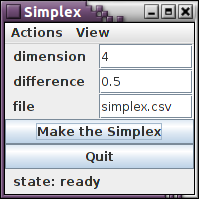
\includegraphics[scale=1]{fig1.png}
\end{minipage}
\hspace{1cm}
\begin{minipage}{0.4\textwidth}
output file 

\begin{verbatim}
0.0;0.0;0.0;1.0
0.0;0.0;0.5;0.5
0.0;0.0;1.0;0.0
0.0;0.5;0.0;0.5
0.0;0.5;0.5;0.0
0.0;1.0;0.0;0.0
0.5;0.0;0.0;0.5
0.5;0.0;0.5;0.0
0.5;0.5;0.0;0.0
1.0;0.0;0.0;0.0
\end{verbatim}
\end{minipage}

\vspace{1cm}

The three entries are: 
\begin{itemize}
\item the dimension (denoted in this document with $N$);
\item the difference (denoted in this document with $d$);
\item and the output file name.
\end{itemize}

The program functions properly if $1/d \in \mathbb{N}_1$.


Under this condition, the output file (named according to the string found in the third text entry box) is created. Each row of the output file is a point on the simplex, that is a $N$-tuple $\{x_1,x_2,...,x_N\}$ such that
\[
\sum_{i=1}^N x_i=1
\]
and each $x_i \in \{0,d,2d,...,1\}$.

If $1/d  \notin \mathbb{N}_1$, a frame inviting you to enter a new value of $d$ appears.

\vspace{1cm}
\centerline{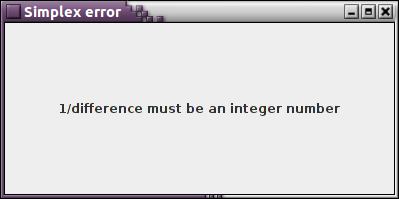
\includegraphics[scale=0.6]{fig2.png}} 
\newpage
The output file can be loaded by your favorite data handling program. 
An easy example is the visualization, rescaling and shifting of points on the $\mathbb{R}^3$ unit simplex.

\section*{Ternary plot}
\centerline{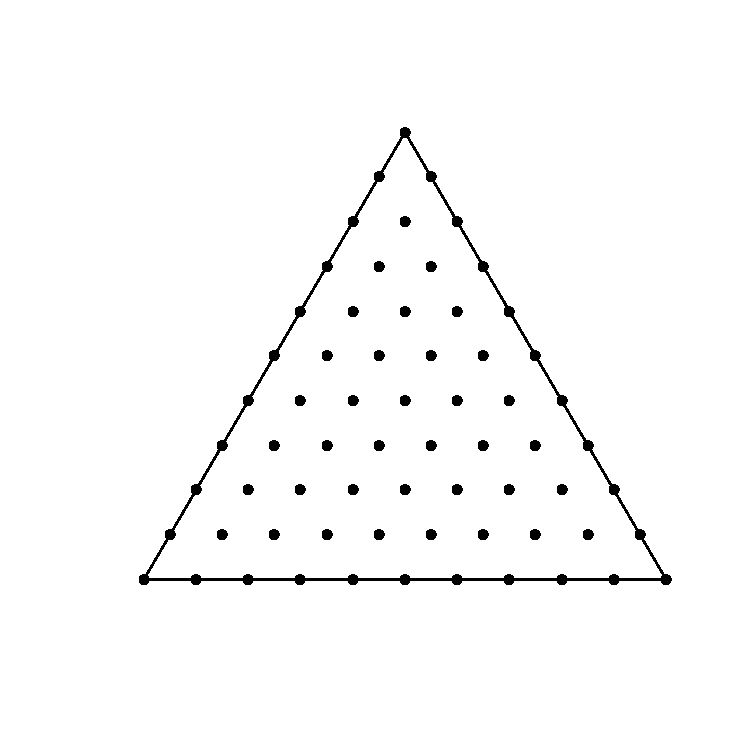
\includegraphics[scale=0.5]{fig1.pdf}}
\vspace{-1cm}
\textbf{Fig. 1:} ternary plot of the data points generated by the program with dimension ($N$) equal to 3 and difference ($d$) equal to 0.1.

\section*{Rescaling and shifting}
The output of the program can be viewed as a matrix $\textbf{S}$ whose number of rows ($Z$) depends on the difference parameter ($d$) and the number of columns is equal to the dimension ($N$). 
We identify each element of this matrix with $s_{z,n}$ so that 
\[
\textbf{S}_{Z\times N}:=[s_{z,n}]
\]
with $z \in {1,2,..,Z}$ and $n \in {1,2,..,N}$.

By definition we have
\[
\textbf{S}_{Z\times N}\textbf{1}_{N\times 1}=\textbf{1}_{Z\times 1}.
\]

Note that
\[
\left[s_{z,n}-\frac{1}{N}\right]\textbf{1}_{N\times 1}=\textbf{0}_{Z\times 1}
\]
and
\[
\max \left(s_{z,n}-\frac{1}{N}\right)=1-\frac{1}{N}.
\]
A further transformation gives 
\[
\left[\frac{s_{z,n}-\frac{1}{N}}{1-\frac{1}{N}}\right]\textbf{1}_{N\times 1}=\textbf{0}_{Z\times 1}
\]
and
\[
\max \left(\frac{s_{z,n}-\frac{1}{N}}{1-\frac{1}{N}}\right)=1.
\]
If we rescale again by the factor $2d$ we obtain
\[
\left[\left(\frac{s_{z,n}-\frac{1}{N}}{1-\frac{1}{N}}\right)2d\right]\textbf{1}_{N\times 1}=\textbf{0}_{Z\times 1}
\]
and
\[
\max \left(\frac{s_{z,n}-\frac{1}{N}}{1-\frac{1}{N}}\right)2d=2d.
\]


Let us define
\[
\textbf{D}_{Z\times N}:=[d_{z,n}]=\left[\left(\frac{s_{z,n}-\frac{1}{N}}{1-\frac{1}{N}}\right)2d\right].
\]
Select a point on the simplex (a row of $\textbf{S}_{Z\times N}$). Let us denote it by $\textbf{s}_{z^*}$.

Fig. 2 shows how the set of points 
\[
\textbf{s}_{z^*}+\textbf{d}_{z}
\]
is in the neighborhood of $\textbf{s}_{z^*}$ (if $\textbf{s}_{z^*}$ lies in the simplex ``boundaries'', the $z$s for which the elements of $\textbf{s}_{z^*}+\textbf{d}_{z}$ fall outside the $[0,1]$ interval must be discarded). 

\centerline{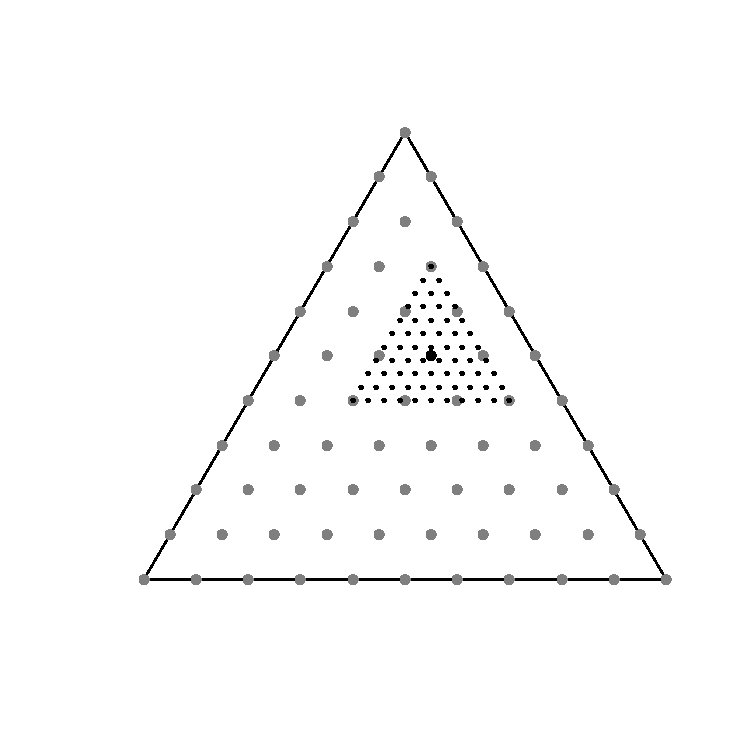
\includegraphics[scale=0.5]{fig2.pdf}}
\vspace{-1cm}
\textbf{FIG. 2:} a rescaled an shifted set of points.

\newpage
\end{document}
